% !TEX root = aata.tex
%%%%(c)
%%%%(c)  This file is a portion of the source for the textbook
%%%%(c)
%%%%(c)    Abstract Algebra: Theory and Applications
%%%%(c)    Copyright 1997 by Thomas W. Judson
%%%%(c)
%%%%(c)  See the file COPYING.txt for copying conditions
%%%%(c)
%%%%(c)
\chap{Galois Theory}{galois}
 
 
A classic problem of algebra has been to find the solutions of a polynomial equation.  The solution to the quadratic equation was known in antiquity.  Italian mathematicians found general solutions to the
general cubic and quartic equations in the sixteenth century; however,  attempts to solve the general fifth-degree, or quintic, polynomial were repulsed for the next three hundred years. Certainly, equations such as $x^5 - 1 = 0$ or $x^6 - x^3 - 6 = 0$ could be solved, but no solution like the quadratic formula was found for the general quintic, 
\[
a x^5 + b x^4 +c x^3 + d x^2 + e x + f = 0.
\]
Finally, at the beginning of the nineteenth century, Ruffini and Abel both found quintics that could not be solved with any formula.  It was Galois, however, who provided the full explanation by showing which
polynomials could and could not be solved by formulas.  He discovered the connection between groups and field extensions.  Galois theory demonstrates the strong interdependence of group and field theory, and has had far-reaching implications beyond its original purpose.  
 
In this chapter we will prove the Fundamental Theorem of Galois Theory.  This result will be used to establish the insolvability of the quintic and to prove the Fundamental Theorem of Algebra. 


\section{Field Automorphisms}
 
Our first task is to establish a link between group theory and field theory by examining automorphisms of fields.
 
\begin{proposition}
The set of all automorphisms of a field $F$ is a group under composition of functions.
\end{proposition}
 
\begin{proof}
If $\sigma$ and $\tau$ are automorphisms of $E$, then so are $\sigma \tau$ and $\sigma^{-1}$.  The identity is certainly an automorphism; hence, the set of all automorphisms of a field $F$ is indeed a group.
\end{proof}

\begin{proposition}
Let $E$ be a field extension of $F$.  Then the set of all automorphisms of $E$ that fix $F$ elementwise is a group; that is, the set of all automorphisms $\sigma : E \rightarrow E$ such that $\sigma( \alpha ) =
\alpha$ for all $\alpha \in F$ is a group.  
\end{proposition}

\begin{proof}
We need only show that the set of automorphisms of $E$ that fix $F$ elementwise is a subgroup of the group of all automorphisms of $E$.  Let $\sigma$ and $\tau$ be two automorphisms of $E$ such that $\sigma( \alpha ) = \alpha$ and $\tau( \alpha ) = \alpha$ for all $\alpha \in F$.  Then $\sigma \tau( \alpha ) = \sigma( \alpha) = \alpha$ and  $\sigma^{-1}( \alpha ) = \alpha$.   Since the identity fixes every  element of $E$, the set of automorphisms of $E$ that leave elements of  $F$ fixed is a subgroup of the entire group of automorphisms of $E$. 
\end{proof}

\medskip

Let $E$ be a field extension of $F$.  We will denote the full group of automorphisms of $E$ by $\aut(E)$.  We define the \boldemph{Galois group\/}\index{Group!Galois}\index{Galois group} of $E$ over $F$ to be
the group of automorphisms of $E$ that fix $F$ elementwise; that is,
\[
G(E/F)\label{notegalois} = \{ \sigma \in \aut(E) : \sigma(\alpha)
=
\alpha \mbox{ for all $\alpha \in F$} \}.
\] 
If $f(x)$ is a polynomial in $F[x]$ and $E$ is the splitting field of $f(x)$ over $F$, then we define the Galois group of $f(x)$ to be $G(E/F)$. 


\begin{example}{complex_conj}
Complex conjugation, defined by $\sigma : a + bi \mapsto a - bi$, is an automorphism of the complex numbers.  Since 
\[
\sigma(a) = \sigma(a + 0i) = a - 0i = a,
\]
the automorphism defined by complex conjugation must be in $G( {\mathbb C} / {\mathbb R} )$. 
\end{example}


\begin{example}{Q_sqrt5}
Consider the fields ${\mathbb Q} \subset {\mathbb Q}(\sqrt{5}\, ) \subset {\mathbb Q}( \sqrt{3}, \sqrt{5}\, )$.  Then for $a, b \in {\mathbb Q}( \sqrt{5}\, )$,
\[
\sigma( a + b \sqrt{3}\, ) = a - b \sqrt{3}
\]
is an automorphism of ${\mathbb Q}(\sqrt{3}, \sqrt{5}\, )$ leaving ${\mathbb Q}( \sqrt{5}\, )$ fixed.  Similarly,
\[
\tau( a + b \sqrt{5}\, ) = a - b \sqrt{5}
\]
is an automorphism of ${\mathbb Q}(\sqrt{3}, \sqrt{5}\, )$ leaving ${\mathbb Q}( \sqrt{3}\, )$ fixed. The automorphism $\mu = \sigma \tau$ moves both $\sqrt{3}$ and $\sqrt{5}$.  It will soon be clear that $\{ id, \sigma, \tau, \mu  \}$ is the Galois group of ${\mathbb Q}(\sqrt{3}, \sqrt{5}\, )$ over ${\mathbb Q}$. The following table shows that this group is isomorphic to ${\mathbb Z}_2 \times {\mathbb Z}_2$.  
\begin{center}
\begin{tabular}{c|cccc}
   & $id$ & $\sigma$ & $\tau$ & $\mu$ \\
\hline
$id$  & $id$ & $\sigma$ & $\tau$ & $\mu$ \\
$\sigma$ & $\sigma$ & $id$ & $\mu$ & $\tau$ \\
$\tau$ & $\tau$ & $\mu$ & $id$ & $\sigma$ \\
$\mu$ & $\mu$ & $\tau$ & $\sigma$ & $id$
\end{tabular}
\end{center}
We may also regard the field ${\mathbb Q}( \sqrt{3}, \sqrt{5}\, )$ as a vector space over ${\mathbb Q}$ that has basis $\{ 1, \sqrt{3}, \sqrt{5}, \sqrt{15}\, \}$.  It is no coincidence that $|G( {\mathbb Q}( \sqrt{3},
\sqrt{5}\, ) /{\mathbb Q})| = [{\mathbb Q}(\sqrt{3}, \sqrt{5}\, ):{\mathbb Q})] = 4$.
\end{example} 
 
\begin{proposition}\label{galois:roots_permute_prop}
Let $E$ be a field extension of $F$ and $f(x)$ be a polynomial in $F[x]$. Then any automorphism in $G(E/F)$ defines a permutation of the roots of $f(x)$ that lie in $E$. 
\end{proposition}
 
\begin{proof}
Let 
\[
f(x) = a_0 + a_1 x + a_2 x^2 + \cdots + a_n x^n
\]
and suppose that $\alpha \in E$ is a zero of $f(x)$. Then for $\sigma \in G(E/F)$,
\begin{align*}
0 & = \sigma( 0 ) \\
& = \sigma( f( \alpha )) \\
& = \sigma(a_0 + a_1\alpha + a_2 \alpha^2 + \cdots + a_n \alpha^n) \\
& = a_0 + a_1 \sigma(\alpha) + a_2 [\sigma(\alpha)]^2 + \cdots + a_n
[\sigma(\alpha)]^n;
\end{align*} 
therefore, $\sigma( \alpha )$ is also a zero of $f(x)$.
\end{proof}

\medskip
 
Let $E$ be an algebraic extension of a field $F$.  Two elements $\alpha, \beta \in E$ are \boldemph{conjugate}\index{Conjugate elements} over $F$ if they have the same minimal polynomial. For example, in the field ${\mathbb Q}( \sqrt{2}\, )$ the elements $\sqrt{2}$ and $-\sqrt{2}$ are conjugate over ${\mathbb Q}$ since they are both roots of the irreducible polynomial $x^2 - 2$.  
 
A converse of the last proposition exists. The proof follows directly from Lemma~\ref{fields:isomorph_lemma}. 

\begin{proposition}
If $\alpha$ and $\beta$ are conjugate over $F$, there exists an isomorphism $\sigma : F( \alpha ) \rightarrow F( \beta )$ such that $\sigma$ is the identity when restricted to~$F$.
\end{proposition}

\begin{theorem}\label{galois:extension_order_theorem}
Let $f(x)$ be a polynomial in $F[x]$ and suppose that $E$ is the splitting field for $f(x)$ over $F$.  If $f(x)$ has no repeated roots, then 
\[
|G(E/F)| = [E:F].
\]
\end{theorem}
 
\begin{proof}
We will use mathematical induction on the degree of $f(x)$.  If the degree of $f(x)$ is 0 or 1, then $E = F$ and there is nothing to show.  Assume
that the result holds for all polynomials of degree $k$ with $0 \leq k < n$.  Suppose that the degree of $f(x)$ is $n$.  Let $p(x)$ be an irreducible factor of $f(x)$ of degree $r$.  Since all of the roots of $p(x)$ are in $E$, we can choose one of these roots, say $\alpha$, so that $F \subset F( \alpha ) \subset E$.  Then
\[
[E: F(\alpha)] = n/r \quad \text{and} \quad [F(\alpha): F] = r.
\]
If $\beta$ is any other root of $p(x)$, then $F \subset F( \beta ) \subset E$.  By Lemma~\ref{fields:isomorph_lemma}, there exists a unique isomorphism $\sigma: F( \alpha ) \rightarrow F( \beta )$ for each such $\beta$ that fixes $F$ elementwise.  Since $E$ is a splitting field of $F(\beta)$, there are exactly $r$ such isomorphisms.  For each of these automorphisms, we can use our induction hypothesis on $[E: F(\alpha)] = n/r < n$ to conclude that
\[
|G(E/F(\alpha))| = [E:F(\alpha)].
\]
Consequently, there are
\[
[E:F] = [E:F(\alpha)] [F( \alpha):F] = n
\]
possible automorphisms of $E$ that fix $F$, or $|G(E/F)| = [E:F]$.

%\paragraph{Original Proof}
%
%
%The proof is similar to the proof of Theorem~\ref{fields:isomorph_extension_theorem}.  We will use mathematical induction on the degree of $f(x)$.  If the degree of $f(x)$ is 0 or 1, then $E = F$ and there is nothing to show.  Assume
%that the result holds for all polynomials of degree $k$ with $0 \leq k < n$.  Suppose that the degree of $f(x)$ is $n$.  Let $p(x)$ be an irreducible factor of $f(x)$ of degree $r$.  Since all of the roots of $p(x)$ are in $E$, we can choose one of
%these roots, say $\alpha$, so that $F \subset F( \alpha ) \subset E$.  If $\beta$ is any other root of $p(x)$, then $F \subset F( \beta ) \subset E$.  By Lemma~\ref{fields:isomorph_lemma}, there exists a unique isomorphism $\overline{\sigma}: F( \alpha ) \rightarrow F( \beta )$ for each such $\beta$ that fixes $F$ elementwise.  Since $E$ is a splitting field of $F(\beta)$, there are exactly $r$ such isomorphisms.  We can factor
%$p(x)$ in $F(\alpha)$ as $p(x) = (x - \alpha) q(x)$.  The degree of $q(x)$ is less than $r$.  Since we know that $E$ is the  splitting field of $q(x)$ over $F(\alpha)$, we can apply
%the induction  hypothesis to conclude that 
%\[
%|G(E/F(\alpha))| = [E:F(\alpha)].
%\]
%Consequently, there are
%\[
%[E:F] = [E:F(\alpha)] [F( \alpha):F]
%\]
%possible automorphisms of $E$ that fix $F$, or $|G(E/F)| = [E:F]$.
\end{proof}

%Proof fixed---I hope.  TWJ 24/4/2013
 
\begin{corollary}
Let $F$ be a finite field with a finite extension $E$ such that $[E:F]=k$. Then $G(E/F)$ is cyclic of order $k$.
\end{corollary}
%Corrected statement of the corollary.  Suggested by K. Wenholz. - TWJ 5/15/2012

\begin{proof}
Let $p$ be the characteristic of $E$ and $F$ and assume that the orders of $E$ and $F$ are $p^m$ and $p^n$, respectively.  Then $nk = m$.  We can also assume that $E$ is the splitting field of $x^{p^m} - x$
over a subfield of order $p$.  Therefore, $E$ must also be the splitting field of $x^{p^m} - x$ over $F$.  Applying Theorem~\ref{galois:extension_order_theorem}, we find that $|G(E/F)| = k$.     

To prove that $G(E/F)$ is cyclic, we must find a generator for $G(E/F)$.  Let $\sigma : E \rightarrow E$ be defined by $\sigma(\alpha) = \alpha^{p^n}$.  We claim that $\sigma$ is the element in $G(E/F)$ that
we are seeking.  We first need to show that $\sigma$ is in $\aut(E)$.  If $\alpha$ and $\beta$ are in $E$,   
\[
\sigma(\alpha + \beta) = (\alpha + \beta)^{p^n}
= \alpha^{p^n} + \beta^{p^n} = \sigma(\alpha) + \sigma(\beta)
\]
by Lemma \ref{finite:freshmans_dream}.  Also, it is easy to show that $\sigma(\alpha \beta) = \sigma( \alpha ) \sigma( \beta )$. Since $\sigma$ is a nonzero homomorphism of fields, it must be injective.  It must also be onto, since $E$ is a finite field.  We know that $\sigma$ must be in $G(E/F)$, since $F$ is the splitting field of $x^{p^n} - x$ over the base field of order $p$. This means that $\sigma$ leaves every element in $F$ fixed.  Finally, we must show that the order of $\sigma$ is $k$. By Theorem~\ref{galois:extension_order_theorem}, we know that $\sigma^k( \alpha ) = \alpha^{p^k} = \alpha$ is the identity of $G( E/F)$.  However, $\sigma^r$ cannot be the identity for $1 \leq r < k$; otherwise, $x^{p^{rk}} - x$ would have $p^m$ roots, which is impossible. 
\end{proof}
 

\begin{example}{galois_group_35}
We can now confirm that the Galois group of ${\mathbb Q}( \sqrt{3},
\sqrt{5}\, )$ over ${\mathbb Q}$ in Example~\ref{example:galois:Q_sqrt5} is indeed isomorphic to
${\mathbb Z}_2 \times {\mathbb Z}_2$.  Certainly the group $H = \{ id,
\sigma, \tau, \mu \}$ is a subgroup of $G({\mathbb Q}( \sqrt{3}, \sqrt{5}\,
)/{\mathbb Q})$; however,  $H$ must be all of $G({\mathbb Q}( \sqrt{3},
\sqrt{5}\, )/{\mathbb Q})$, since  
\[
|H| = [{\mathbb Q}( \sqrt{3}, \sqrt{5}\, ):{\mathbb Q}] = |G({\mathbb Q}(
\sqrt{3}, \sqrt{5}\, )/{\mathbb Q})| = 4.
\]
\end{example}
 

\begin{example}{galois_group_x4}
Let us compute the Galois group of 
\[
f(x) = x^4 + x^3 + x^2 + x + 1
\]
over ${\mathbb Q}$. We know that $f(x)$ is irreducible by Exercise~\ref{poly:Cyclotomic_Polynomials} in
Chapter~\ref{poly}.  Furthermore, since $(x -1)f(x) = x^5 -1$, we can use
DeMoivre's Theorem to determine that the roots of $f(x)$ are
$\omega^i$,  where  $i = 1, \ldots, 4$ and 
\[
\omega = \cos(2 \pi / 5 ) + i \sin(2 \pi / 5 ).
\]
Hence, the splitting field of $f(x)$ must be ${\mathbb Q}(\omega)$.  We 
can define automorphisms $\sigma_i$ of ${\mathbb Q}(\omega )$ by 
$\sigma_i( \omega ) = \omega^i$ for $i = 1, \ldots, 4$.  It is easy to check
that these are indeed distinct automorphisms in $G( {\mathbb Q}( \omega)
/ {\mathbb Q} )$.  Since 
\[
[{\mathbb Q}( \omega) : {\mathbb Q}] = | G( {\mathbb Q}(
\omega) / {\mathbb Q})| = 4,
\]
the $\sigma_i$'s must be all of $G( {\mathbb
Q}( \omega) / {\mathbb Q} )$. Therefore, $G({\mathbb Q}( \omega) / {\mathbb Q})
\cong {\mathbb Z}_4$ since $\omega$ is a generator for the Galois group. 
\end{example}
 
 
 
\subsection*{Separable Extensions}
 
 
Many of the results that we have just proven depend on the fact that a
polynomial $f(x)$ in $F[x]$ has no repeated roots in its splitting
field. It is evident that we need to know exactly when a
polynomial factors into distinct linear factors in its splitting
field. Let $E$ be the splitting field of a polynomial $f(x)$ in $F[x]$.
Suppose that $f(x)$ factors over $E$ as
\[
f(x) = (x - \alpha_1)^{n_1} (x - \alpha_2)^{n_2} \cdots (x -
\alpha_r)^{n_r} = \prod_{i=1}^{r} (x - \alpha_i)^{n_i}.
\]
We define the \boldemph{multiplicity}\index{Multiplicity of a
root}\index{Zero!multiplicity of} of a root $\alpha_i$ of $f(x)$ to be
$n_i$.  A root with multiplicity 1 is called a \boldemph{simple
root}\index{Simple root}. Recall that a polynomial $f(x) \in F[x]$ of
degree $n$ is \boldemph{separable}\index{Polynomial!separable} if it has
$n$ distinct roots in its splitting field $E$. Equivalently, $f(x)$ is
separable if it factors into distinct linear factors over $E[x]$.
An extension $E$ of $F$ is a \boldemph{separable
extension}\index{Extension!separable} of $F$ if every element in $E$
is the root of a separable polynomial in $F[x]$. Also recall that
$f(x)$ is separable if and only if $\gcd( f(x), f'(x)) = 1$
(Lemma~\ref{finite:separable_derivative_lemma}). 
 
% 2010/05/18 R Beezer, replaced "over F[x]" by "over F"
\begin{proposition}
Let $f(x)$ be an irreducible polynomial over $F$. If the
characteristic of $F$ is $0$, then $f(x)$ is separable.  If the
characteristic of $F$ is $p$ and $f(x) \neq g(x^p)$ for some $g(x)$
in $F[x]$, then $f(x)$ is also separable.
\end{proposition}
 
 
\begin{proof}
First assume that ${\rm char } F = 0$. Since $\deg f'(x) < \deg f(x)$ 
and $f(x)$ is irreducible, the only way $\gcd( f(x), f'(x)) \neq 1$ is
if $f'(x)$ is the zero polynomial; however, this is impossible in
a field of characteristic zero. If ${\rm char } F = p$, then $f'(x)$
can be the zero polynomial if every coefficient of $f(x)$ is a
multiple of $p$.  This can happen only if we have a polynomial of the
form $f(x) = a_0 + a_1 x^p + a_2 x^{2p} + \cdots + a_n x^{np}$. 
\end{proof}
 
 
\medskip
 
 
Certainly extensions of a field $F$ of the form $F(\alpha)$ are some
of the easiest to study and understand.  Given a field extension $E$
of $F$, the obvious question to ask is when it is possible to find an
element $\alpha \in E$ such that $E = F( \alpha )$. In this case,
$\alpha$ is called a \boldemph{primitive
element}\index{Element!primitive}\index{Primitive element}. We already
know that primitive elements exist for certain extensions. For example,
\[
{\mathbb Q}( \sqrt{3}, \sqrt{5}\, ) = {\mathbb Q}( \sqrt{3} + \sqrt{5}\, )
\]
and
\[
{\mathbb Q}( \sqrt[3]{5}, \sqrt{5}\, i ) = {\mathbb Q}( \sqrt[6]{5}\, i ).
\]
Corollary~\ref{finite:finite_extension_corollary} tells us that there exists a primitive element for any 
finite extension of a finite field. The next theorem tells us that we 
can often find a primitive element.
 
 
\begin{theorem}[Primitive Element Theorem]\index{Primitive Element
Theorem}\label{galois:primitive_element_theorem}
Let $E$ be a finite separable extension of a field $F$. Then there
exists an $\alpha \in E$ such that $E=F( \alpha )$. 
\end{theorem}
 
 
\begin{proof}
We already know that there is no problem if $F$ is a finite field. 
Suppose that $E$ is a finite extension of an infinite field. We will 
prove the result for $F(\alpha, \beta)$.  The general case easily
follows when we use mathematical induction. Let $f(x)$ and $g(x)$ be  the
minimal polynomials of $\alpha$ and $\beta$, respectively. Let $K$ be
the field in which both $f(x)$ and $g(x)$ split. Suppose that $f(x)$
has zeros $\alpha = \alpha_1, \ldots, \alpha_n$ in $K$ and $g(x)$ has
zeros $\beta = \beta_1, \ldots, \beta_m$ in $K$. All of these zeros
have multiplicity 1, since $E$ is separable over $F$. Since $F$ is
infinite, we can find an $a$ in $F$ such that  
\[
a \neq \frac{\alpha_i - \alpha}{\beta - \beta_j}
\]
for all $i$ and $j$ with $j \neq 1$. Therefore, $a( \beta - \beta_j ) 
\neq \alpha_i - \alpha$. Let $\gamma = \alpha +a \beta$. Then
\[
\gamma = \alpha + a \beta \neq \alpha_i + a \beta_j;
\]
hence, $\gamma - a \beta_j \neq \alpha_i$ for all $i, j$ with $j \neq 1$. 
Define $h(x) \in F( \gamma )[x]$ by $h(x) = f( \gamma - ax)$. Then $h(
\beta ) = f( \alpha ) = 0$. However, $h( \beta_j ) \neq 0$ for $j \neq
1$. Hence, $h(x)$ and $g(x)$ have a single common factor in $F( \gamma
)[x]$; that is, the irreducible polynomial of $\beta$ over $F( \gamma
)$ must be linear, since $\beta$ is the only zero common to both $g(x)$
and $h(x)$. So $\beta \in F( \gamma )$ and $\alpha = \gamma - a \beta$
is in $F( \gamma )$. Hence, $F( \alpha, \beta ) = F( \gamma )$. 
\end{proof}
 
 
 
\section{The Fundamental Theorem}
 
 
The goal of this section is to prove the Fundamental Theorem of	Galois 
Theory. This theorem explains the connection between the subgroups of 
$G(E/F)$ and the intermediate fields between $E$ and $F$.  
 
 
\begin{proposition}
Let $\{\sigma_i : i \in I  \}$ be a  collection of automorphisms of a
field $F$.  Then 
\[
F_{ \{\sigma_i \}    } = \{ a \in F : \sigma_i(a) = a \mbox{
for all $\sigma_i$}  \}\label{noteFixedfield}
\]
is a subfield of $F$.
\end{proposition}
 
 
\begin{proof}
Let $\sigma_i(a) = a$ and $\sigma_i(b)=b$. Then
\[
\sigma_i(a \pm b) = \sigma_i(a) \pm \sigma_i(b) = a \pm b
\]
and
\[
\sigma_i(a b) = \sigma_i(a) \sigma_i(b) = a  b.
\]
If $a \neq 0$, then  $\sigma_i(a^{-1}) = [\sigma_i(a)]^{-1} = a^{-1}$.
Finally, $\sigma_i(0) = 0$ and $\sigma_i(1)=1$ since $\sigma_i$ is an
automorphism.  
\end{proof}
 
\begin{corollary}
Let $F$ be a field and let $G$ be a subgroup of $\aut(F)$. Then 
\[
F_G\label{noteFixedG} = \{ \alpha \in F : \sigma( \alpha ) = \alpha
\mbox{ for all $\sigma \in G$} \}
\]
is a subfield of $F$.
\end{corollary}
 
 
%\medskip
 
 
The subfield $F_{ \{\sigma_i \} }$ of $F$ is called the \boldemph{fixed
field\/}\index{Field!fixed} of $\{ \sigma_i \}$. The field fixed for a
subgroup $G$ of $\aut(F)$ will be denoted by $F_G$. 
 

\begin{example}{}
Let $\sigma : {\mathbb Q}(\sqrt{3}, \sqrt{5}\, ) \rightarrow {\mathbb
Q}(\sqrt{3}, \sqrt{5}\, )$ be the automorphism that maps $\sqrt{3}$ to
$-\sqrt{3}$. Then ${\mathbb Q}( \sqrt{5}\, )$ is the subfield of 
${\mathbb Q}(\sqrt{3}, \sqrt{5}\, )$ left fixed by $\sigma$.
\mbox{\hspace{1in}}
\end{example}
 
 
\begin{proposition}\label{galois:fixed_field_prop}
Let $E$ be a splitting field over $F$ of a separable polynomial.
Then $E_{G(E/F)} = F$.
\end{proposition}
 
 
\begin{proof}
Let $G = G(E/F)$. Clearly, $F \subset E_G \subset E$. Also, $E$ 
must be a splitting field of $E_G$ and $G(E/F) = G(E/E_G)$. By
Theorem~\ref{galois:extension_order_theorem},
\[
|G| = [E: E_G] =[ E:F].
\]
Therefore, $[E_G : F ] =1$. Consequently,  $E_G = F$.
\end{proof}
 
 
\medskip
 
 
A large number of mathematicians first learned Galois theory from
Emil Artin's monograph on the subject [1]. The very clever proof of
the following lemma is due to Artin. 
 
 
\begin{lemma}
Let $G$ be a finite group of automorphisms of $E$ and let $F = E_G$.
Then $[E:F] \leq |G|$.
\end{lemma}
 
 
\begin{proof}
Let $|G| = n$. We must show that any set of $n+1$ elements $\alpha_1,
\ldots, \alpha_{n+1}$ in $E$ is linearly dependent over $F$; that is,
we need to find elements $a_i \in F$, not all zero, such that 
\[
a_1 \alpha_1 + a_2 \alpha_2 + \cdots + a_{n+1} \alpha_{n+1} = 0.
\]
Suppose that $\sigma_1 = id, \sigma_2, \ldots, \sigma_n$ are the
automorphisms in $G$. The homogeneous system of linear
equations 
\begin{align*}
\sigma_1( \alpha_1 ) x_1 + \sigma_1(\alpha_2) x_2 + \cdots +
\sigma_1(\alpha_{n+1} ) x_{n+1} & = 0 \\
\sigma_2( \alpha_1 ) x_1 + \sigma_2(\alpha_2) x_2 + \cdots +
\sigma_2(\alpha_{n+1} ) x_{n+1} & = 0 \\
& \vdots & \\
\sigma_n( \alpha_1 ) x_1 + \sigma_n(\alpha_2) x_2 + \cdots +
\sigma_n(\alpha_{n+1} ) x_{n+1} & = 0
\end{align*}
has more unknowns than equations. From linear algebra we know that
this system has a nontrivial solution, say $x_i = a_i$ for $i = 1, 2,
\ldots, n+1$. Since $\sigma_1$ is the identity, the first equation
translates to
\[
a_1 \alpha_1 +  a_2 \alpha_2  + \cdots + a_{n+1} \alpha_{n+1} = 0.
\]
The problem is that some of the $a_i$'s may be in $E$ but not in $F$. 
We must show that this is impossible.
%Corrected typo.  Suggested by K. Brooks. - TWJ 6/15/2012
 
 
Suppose that at least one of the $a_i$'s is in $E$ but not in $F$. By
rearranging the $\alpha_i$'s we may assume that $a_1$ is nonzero.
Since any nonzero multiple of a solution is also a solution, we can
also assume that $a_1 = 1$. Of all possible solutions fitting this
description, we choose the one with the smallest number of nonzero terms.
Again, by rearranging $\alpha_2, \ldots, \alpha_{n+1}$ if necessary,
we can assume that $a_2$ is in $E$ but not in $F$. Since $F$ is the
subfield of $E$ that is fixed elementwise by $G$, there exists a
$\sigma_i$ in $G$ such that $\sigma_i( a_2 ) \neq a_2$. Applying
$\sigma_i$ to each equation in the system, we end up with the same
homogeneous system, since $G$ is a group. Therefore, $x_1 =
\sigma_i(a_1) = 1$, $x_2 = \sigma_i(a_2)$, $\ldots$, $x_{n+1} =
\sigma_i(a_{n+1} )$ is also a solution of the original system. We know
that a linear combination of two solutions of a homogeneous system is
also a solution; consequently,   
\begin{align*}
x_1 & = 1 -1 = 0 \\
x_2 & = a_2 - \sigma_i(a_2) \\
& \vdots & \\
x_{n+1} & = a_{n+1} - \sigma_i(a_{n+1}) 
\end{align*}
must be another solution of the system. This is a nontrivial solution
because $\sigma_i( a_2 ) \neq a_2$, and has fewer nonzero entries than
our original solution. This is a contradiction, since the number of
nonzero solutions to our original solution was assumed to be minimal.
We can therefore conclude that $a_1 = \cdots = a_{n+1} = 0$.
\end{proof}
 
 
\medskip
 
 
Let $E$ be an algebraic extension of $F$. If every irreducible
polynomial in $F[x]$ with a root in $E$ has all of its roots in
$E$, then $E$ is called a \boldemph{normal
extension}\index{Extension!normal}\index{Normal extension} of $F$;
that is, every irreducible polynomial in $F[x]$ containing a root in
$E$ is the product of linear factors in $E[x]$. 
 
 
\begin{theorem}
Let $E$ be a field extension of $F$. Then the following statements are
equivalent.
\begin{enumerate}
 
\rm \item \it
$E$ is a finite, normal, separable extension of $F$.
 
\rm \item \it
$E$ is a splitting field over $F$ of a separable polynomial.
 
\rm \item \it
$F = E_G$ for some finite group of automorphisms of $E$.
 
\end{enumerate}
\end{theorem}
 
 
\begin{proof}
(1) $\Rightarrow$ (2). 
Let $E$ be a finite, normal, separable extension of $F$. By the
Primitive Element Theorem, we can find an  $\alpha$ in $E$ such that
$E = F(\alpha)$. Let $f(x)$ be the minimal polynomial of $\alpha$ over
$F$. The field $E$ must contain all of the roots of $f(x)$ since it is
a normal extension $F$; hence, $E$ is a splitting field for $f(x)$.
 
 
(2) $\Rightarrow$ (3). 
Let $E$ be the splitting field over $F$ of a separable polynomial. By
Proposition~\ref{galois:fixed_field_prop}, $E_{G(E/F)} = F$. Since $| G(E/F)| = [E:F]$, this is
a finite group. 
 
(3) $\Rightarrow$ (1). 
Let $F = E_G$ for some finite group of automorphisms $G$ of $E$. Since
$[E:F] \leq |G|$, $E$ is a finite extension of $F$. To show that $E$
is a finite, normal extension of  $F$, let $f(x) \in F[x]$ be an
irreducible monic polynomial that has a root $\alpha$ in $E$. We must
show that $f(x)$ is the product of distinct linear factors in $E[x]$.
By Proposition \ref{galois:roots_permute_prop}, automorphisms in $G$ permute the roots of $f(x)$
lying in $E$. Hence, if we let $G$ act on $\alpha$, we can obtain
distinct roots $\alpha_1 = \alpha, \alpha_2, \ldots, \alpha_n$ in $E$.
Let $g(x) = \prod_{i=1}^{n} (x -\alpha_i)$. Then $g(x)$ is separable
over $F$ and $g( \alpha ) = 0$. Any automorphism $\sigma$ in $G$
permutes the factors of $g(x)$ since it permutes these roots; hence,
when $\sigma$ acts on $g(x)$, it must fix the coefficients of $g(x)$.
Therefore, the coefficients of $g(x)$ must be in $F$. Since $\deg g(x)
\leq \deg f(x)$ and $f(x)$ is the minimal polynomial of $\alpha$,
$f(x) = g(x)$.
\end{proof}
 
 
\begin{corollary}
Let $K$ be a field extension of $F$ such that $F = K_G$ for some
finite group of automorphisms $G$ of $K$. Then $G = G(K/F)$. 
\end{corollary}
 
 
\begin{proof}
Since $F = K_G$, $G$ is a subgroup of $G(K/F)$. Hence,
\[
[K : F ]  \leq |G| \leq |G(K/F)| = [K:F].
\]
It follows that $G = G(K/F)$, since they must have the same order.
\end{proof}
 
 
\medskip
 
 
Before we determine the exact correspondence between field extensions
and automorphisms of fields, let us return to a familiar example. 
 

\begin{example}{field_lattice}
In Example \ref{example:galois:Q_sqrt5} we examined the automorphisms of ${\mathbb Q}( \sqrt{3},
\sqrt{5}\, )$ fixing ${\mathbb Q}$. Figure~\ref{Galois1}  compares the
lattice of field extensions of ${\mathbb Q}$ with the lattice of
subgroups of $G( {\mathbb Q}( \sqrt{3}, \sqrt{5}\, ) /{\mathbb Q})$.
The Fundamental Theorem of Galois Theory tells us what the 
relationship is between the two lattices.
\end{example} 
 


\begin{figure}[t]
\begin{center}
\tikzpreface{galois_root3_root5}
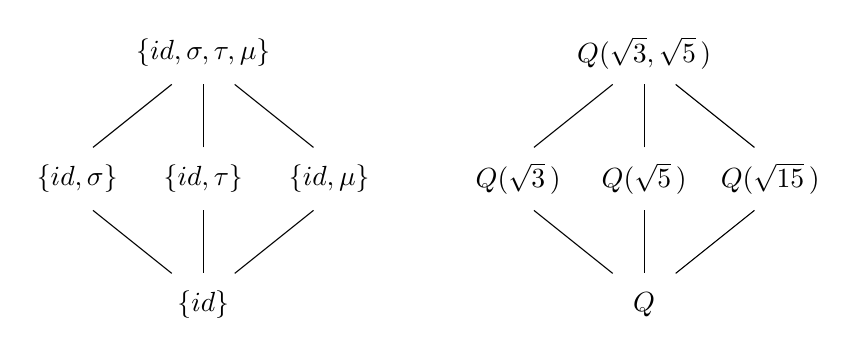
\begin{tikzpicture}[scale=0.8] %Replaced figure with tikz figure and corrected figure - TWJ 8/20/2010

\draw  (2,0.5) -- (2,1.5);
\draw  (2,-0.5) -- (2,-1.5);

\draw  (0.25,0.5) -- (1.5,1.5);
\draw  (0.25,-0.5) -- (1.5,-1.5);
\draw  (3.75,0.5) -- (2.5,1.5);
\draw  (3.75,-0.5) -- (2.5,-1.5);

\draw  (9,0.5) -- (9,1.5);
\draw  (9,-0.5) -- (9,-1.5);

\draw  (7.25,0.5) -- (8.5,1.5);
\draw  (7.25,-0.5) -- (8.5,-1.5);
\draw  (10.75,0.5) -- (9.5,1.5);
\draw  (10.75,-0.5) -- (9.5,-1.5);

\node at (0,0)  {$\{  id, \sigma \}$};
\node at (2,0)  {$\{  id, \tau \}$};
\node at (4,0)  {$\{  id, \mu \}$};
\node at (2,2)  {$\{  id, \sigma, \tau, \mu \}$};
\node at (2,-2)  {$\{  id \}$};

\node at (7,0)  {${\mathbb Q}(\sqrt{3}\, )$};
\node at (9,0)  {${\mathbb Q}(\sqrt{5}\, )$};
\node at (11,0)  {${\mathbb Q}(\sqrt{15}\, )$};
\node at (9,2)  {${\mathbb Q}(\sqrt{3}, \sqrt{5}\, )$};
\node at (9,-2)  {${\mathbb Q}$};


\end{tikzpicture}
\end{center}
\caption{$G({\mathbb Q}( \protect\sqrt{3}, \protect\sqrt{5}\, ) / {\mathbb
Q})$} 
\label{Galois1}
\end{figure}
 
 
We are now ready to state and prove the Fundamental Theorem of Galois
Theory.
 
 
\begin{theorem}
\textbf{(Fundamental Theorem of Galois Theory)}\index{Fundamental
Theorem!of Galois Theory}\label{galois:fundamental_theorem}
Let $F$ be a finite field or a field of characteristic zero. If $E$ is
a finite normal extension of $F$ with Galois group $G(E/F)$, then the
following statements are true. 
\begin{enumerate}
 
\rm \item \it
The map $K \mapsto G(E/K)$ is a bijection of subfields $K$ of $E$
containing $F$ with the subgroups of $G(E/F)$.  
 
\rm \item \it 
If $F \subset K \subset E$, then 
\[
[E:K] = |G(E/K)|
\mbox{ and }
[K:F] = [G(E/F):G(E/K)].
\]
 
\rm \item \it 
$F \subset K \subset L \subset E$ if and only if $\{ id \} \subset
G(E/L) \subset G(E/K) \subset G(E/F)$.
 
 
\rm \item \it 
$K$ is a normal extension of $F$ if and only if $G(E/K)$ is a normal 
subgroup of $G( E/F)$. In this case
\[
G(K/F) \cong G(E/F) / G( E/K ).
\] 
 
\end{enumerate}
\end{theorem}
 
 
\begin{proof}
(1)
Suppose that $G(E/K) = G(E/L) = G$. Both $K$ and $L$ are fixed fields 
of $G$; hence, $K=L$ and the map defined by $K \mapsto G(E/K)$ is
one-to-one. To show that the map is onto, let $G$ be a subgroup of
$G(E/F)$ and $K$ be the field fixed by $G$. Then $F \subset K \subset
E$; consequently, $E$ is a normal extension of $K$. Thus, $G(E/K) = G$
and the map $K \mapsto G(E/K)$ is a bijection. 
 
 
(2)
By Theorem \ref{galois:extension_order_theorem}, $|G(E/K)| = [E:K]$; therefore, 
\[
|G(E/F)| = [G(E/F):G(E/K)] \cdot |G(E/K)| = [E:F] = [E:K][K:F].
\]
Thus, $[K:F] = [G(E/F):G(E/K)]$.
 
 
(3)
Statement (3) is illustrated in Figure~\ref{Galois2}.
We leave the proof of this property as an exercise.
 
\begin{figure}[htb]
\begin{center}
\tikzpreface{galois_correspondence}
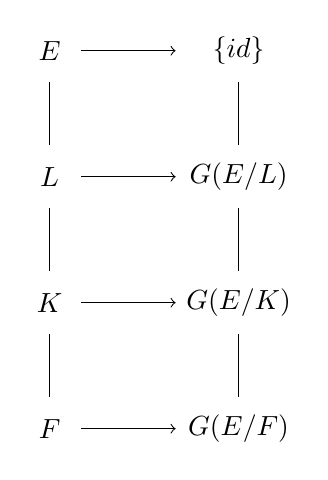
\begin{tikzpicture}[scale=0.8] %Replaced figure with tikz figure and corrected figure - TWJ 8/20/2010

\draw  (0,0.5) -- (0,1.5);
\draw  (0,2.5) -- (0,3.5);
\draw  (0,4.5) -- (0,5.5);

\draw  (3,0.5) -- (3,1.5);
\draw  (3,2.5) -- (3,3.5);
\draw  (3,4.5) -- (3,5.5);

\draw [->] (0.5,0) -- (2,0);
\draw [->] (0.5,2) -- (2,2);
\draw [->] (0.5,4) -- (2,4);
\draw [->] (0.5,6) -- (2,6);

\node at (0,0)  {$F$};
\node at (3,0)  {$G(E/F)$};

\node at (0,2)  {$K$};
\node at (3,2)  {$G(E/K)$};

\node at (0,4)  {$L$};
\node at (3,4)  {$G(E/L)$};

\node at (0,6)  {$E$};
\node at (3,6)  {$\{  id \}$};

\end{tikzpicture}
\end{center}
\caption{Subgroups of $G(E/F)$ and subfields of $E$} 
\label{Galois2}
\end{figure}
 
 
(4)
This part takes a little more work. Let $K$ be a normal extension of
$F$. If $\sigma$ is in $G(E/F)$ and $\tau$ is in $G(E/K)$, we need to
show that $\sigma^{-1} \tau \sigma$ is in $G(E/K)$; that is, we need
to show that $\sigma^{-1} \tau \sigma( \alpha) = \alpha$ for all
$\alpha \in K$.	Suppose that $f(x)$ is the minimal polynomial of
$\alpha$ over $F$. Then $\sigma( \alpha )$ is also a root of
$f(x)$ lying in $K$, since $K$ is a normal extension of $F$. Hence,
$\tau( \sigma( \alpha )) = \sigma( \alpha )$ or $\sigma^{-1} \tau 
\sigma( \alpha) = \alpha$.
 
 
Conversely, let $G(E/K)$ be a normal subgroup of $G(E/F)$. We need to
show that $F = K_{G(K/F)}$. Let $\tau \in G(E/K)$. For all $\sigma
\in G(E/F)$ there exists a $\overline{\tau} \in G(E/K)$ such that
$\tau \sigma = \sigma \overline{\tau}$.  Consequently, for all $\alpha
\in K$
\[
\tau( \sigma( \alpha ) )
= \sigma( \overline{\tau}( \alpha ) )
= \sigma( \alpha );
\]
hence, $\sigma( \alpha )$ must be in the fixed field of $G(E/K)$.
Let $\overline{\sigma}$ be the restriction of $\sigma$ to $K$. Then
$\overline{\sigma}$ is an automorphism of $K$ fixing $F$, since
$\sigma( \alpha ) \in K$ for all $\alpha \in K$; hence,
$\overline{\sigma} \in G(K/F)$. Next, we will show that the fixed
field of $G(K/F)$ is $F$. Let $\beta$ be an element in $K$ that is
fixed by all automorphisms in $G(K/F)$.  In particular,
$\overline{\sigma}(\beta) = \beta$ for all $\sigma \in G(E/F)$. 
Therefore, $\beta$ belongs to the fixed field $F$ of $G(E/F)$.
 
 
Finally, we must show that when $K$ is a normal extension of $F$, 
\[
G(K/F) \cong G(E/F) / G(E/K).
\]
For $\sigma \in G(E/F)$, let $\sigma_K$ be the automorphism of $K$
obtained by restricting $\sigma$ to $K$. Since $K$ is a normal
extension, the argument in the preceding paragraph shows that
$\sigma_K \in G( K/F)$. Consequently, we have a map \mbox{$\phi:G(E/F)
\rightarrow G(K/F)$} defined by $\sigma \mapsto \sigma_K$. This map is
a group homomorphism since
\[
\phi( \sigma \tau ) 
= (\sigma \tau)_K 
= \sigma_K \tau_K 
= \phi( \sigma) \phi( \tau ).
\]
The kernel of $\phi$ is $G(E/K)$.  By (2), 
\[
|G(E/F)| / |G(E/K)| = [K:F] = |G(K/F)|.
\]
Hence, the image of $\phi$ is $G(K/F)$ and $\phi$ is 
onto. Applying the First Isomorphism Theorem, we have
\[
G(K/F) \cong G(E/F) / G( E/K ).
\]
\end{proof}
 
 

\begin{example}{galois_x4-2}
In this example we will illustrate the Fundamental Theorem of Galois
Theory by determining the lattice of subgroups of the Galois group of
$f(x) = x^4 - 2$. We will compare this lattice to the lattice of field
extensions of ${\mathbb Q}$ that are contained in the splitting field of
$x^4-2$. The splitting field of $f(x)$ is ${\mathbb Q}( \sqrt[4]{2}, i
)$. To see this, notice that $f(x)$ factors as $(x^2 +
\sqrt{2}\, )(x^2 - \sqrt{2}\, )$; hence, the roots of $f(x)$ are $\pm
\sqrt[4]{2}$ and $\pm \sqrt[4]{2}\, i$. We first adjoin the root
$\sqrt[4]{2}$ to ${\mathbb Q}$ and then adjoin the root $i$ of $x^2 + 1$
to ${\mathbb Q}(\sqrt[4]{2}\, )$. The splitting field of $f(x)$ is then
${\mathbb Q}(\sqrt[4]{2}\, )(i) = {\mathbb Q}( \sqrt[4]{2}, i )$. 
 
 
Since $[ {\mathbb Q}( \sqrt[4]{2}\, ) : {\mathbb Q}] = 4$ and $i$ is not in
${\mathbb Q}( \sqrt[4]{2}\, )$, it must be the case that $[ {\mathbb Q}(
\sqrt[4]{2}, i ): {\mathbb Q}(\sqrt[4]{2}\, )] = 2$. Hence, $[ {\mathbb Q}(
\sqrt[4]{2}, i ):{\mathbb Q}] = 8$. The set
\[
\{ 1, \sqrt[4]{2}, (\sqrt[4]{2}\, )^2, (\sqrt[4]{2}\, )^3, i, i
\sqrt[4]{2}, i (\sqrt[4]{2}\, )^2, i(\sqrt[4]{2}\, )^3 \}
\]
is a basis of ${\mathbb Q}( \sqrt[4]{2}, i )$ over ${\mathbb Q}$. The
lattice of field extensions of ${\mathbb Q}$ contained in ${\mathbb Q}(
\sqrt[4]{2}, i)$ is illustrated in Figure~\ref{Galois3}(a).
 
%Corrected the automorphism sigma.  Suggested by R. Beezer. - TWJ 4/14/2011
The Galois group $G$ of $f(x)$ must be of order 8. Let $\sigma$ be the
automorphism defined by $\sigma( \sqrt[4]{2}\, ) = i \sqrt[4]{2}$ and
$\sigma( i ) = i$, and $\tau$ be the automorphism defined by complex
conjugation; that is, $\tau(i ) = -i$. Then $G$ has an element of
order 4 and an element of order 2. It is easy to verify by direct
computation that the elements of $G$ are $\{ id, \sigma, \sigma^2, 
\sigma^3, \tau, \sigma \tau, \sigma^2 \tau, \sigma^3 \tau \}$ and that
the relations $\tau^2 = id$, $\sigma^4 = id$, and $\tau \sigma \tau =
\sigma^{-1}$ are satisfied; hence, $G$ must be isomorphic to $D_4$.
The lattice of subgroups of $G$ is illustrated in Figure~\ref{Galois3}(b).
\end{example}
 
\begin{figure}[htb]
\begin{center}

\tikzpreface{galois_fourth_root2}
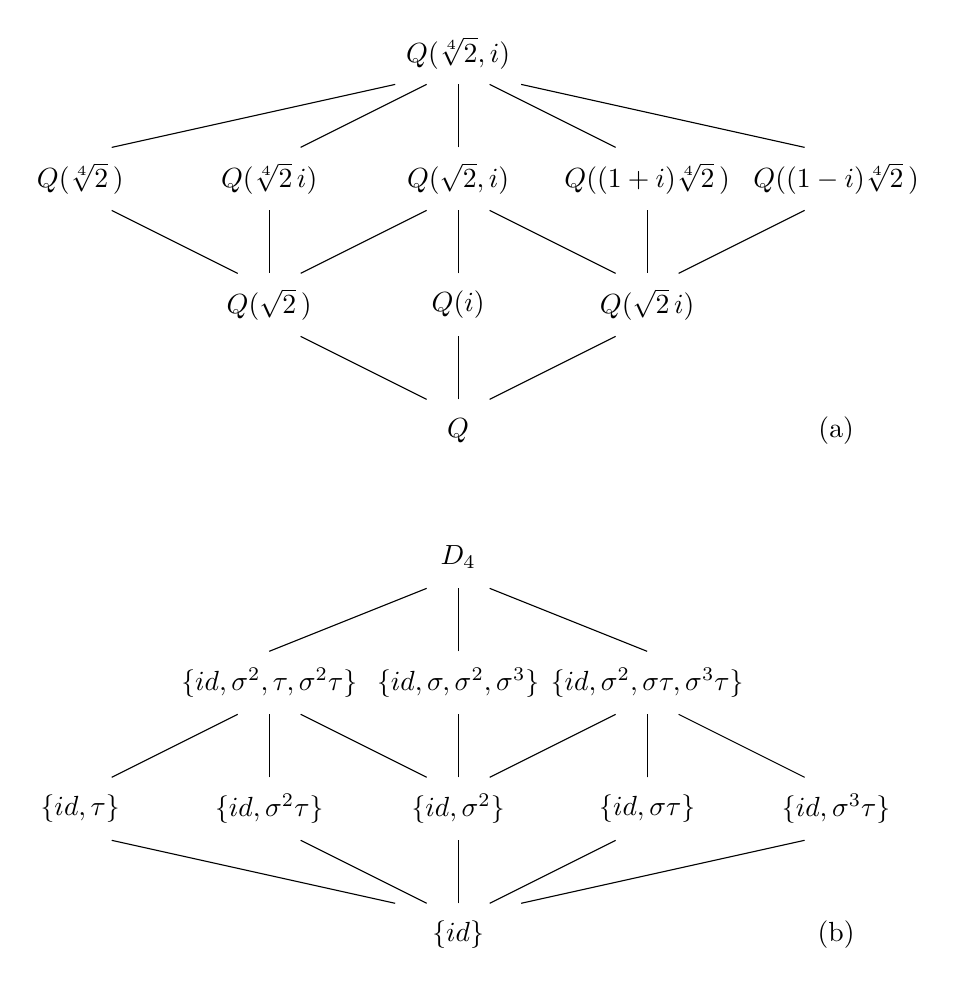
\begin{tikzpicture}[scale=0.8] %Replaced figure with tikz figure and corrected figure - TWJ 8/20/2010

\draw  (-1,0.5) -- (-5.5,1.5);
\draw  (-0.5,0.5) -- (-2.5,1.5);
\draw  (0,0.5) -- (0,1.5);
\draw  (0.5,0.5) -- (2.5,1.5);
\draw  (1,0.5) -- (5.5,1.5);


\draw  (-5.5,2.5) -- (-3.5,3.5);
\draw  (-3,2.5) -- (-3,3.5);
\draw  (-0.5,2.5) -- (-2.5,3.5);
\draw  (0,2.5) -- (0,3.5);
\draw  (5.5,2.5) -- (3.5,3.5);
\draw  (3,2.5) -- (3,3.5);
\draw  (0.5,2.5) -- (2.5,3.5);
\draw  (3,2.5) -- (3,3.5);

\draw  (-3,4.5) -- (-0.5,5.5);
\draw  (0,4.5) -- (0,5.5);
\draw  (3,4.5) -- (0.5,5.5);

\node at (0,0)  {$\{  id \}$};
\node at (-6,2)  {$\{  id, \tau \}$};
\node at (-3,2)  {$\{  id, \sigma^2 \tau \}$};
\node at (0,2)  {$\{  id, \sigma^2 \}$};
\node at (3,2)  {$\{  id, \sigma \tau \}$};
\node at (6,2)  {$\{  id, \sigma^3 \tau \}$};
\node at (-3,4)  {$\{  id, \sigma^2, \tau, \sigma^2 \tau \}$};
\node at (0,4)  {$\{  id, \sigma, \sigma^2, \sigma^3 \}$};
\node at (3,4)  {$\{  id, \sigma^2, \sigma \tau, \sigma^3 \tau \}$};
\node at (0,6)  {$D_4$};
\node at (6,0) {(b)};

\draw  (-0.5,8.5) -- (-2.5,9.5);
\draw  (0,8.5) -- (0,9.5);
\draw  (0.5,8.5) -- (2.5,9.5);

\draw  (-5.5,11.5) -- (-3.5,10.5);
\draw  (-3,11.5) -- (-3,10.5);
\draw  (-0.5,11.5) -- (-2.5,10.5);

\draw  (0,10.5) -- (0,11.5);

\draw  (5.5,11.5) -- (3.5,10.5);
\draw  (3,11.5) -- (3,10.5);
\draw  (0.5,11.5) -- (2.5,10.5);

\draw  (-5.5,12.5) -- (-1,13.5);
\draw  (-2.5,12.5) -- (-0.5,13.5);
\draw  (0,12.5) -- (0,13.5);
\draw  (2.5,12.5) -- (0.5,13.5);
\draw  (5.5,12.5) -- (1,13.5);

\node at (0,8)  {${\mathbb Q}$};
\node at (-3,10)  {${\mathbb Q}(\sqrt{2}\, )$};
\node at (0,10)  {${\mathbb Q}(i)$};
\node at (3,10)  {${\mathbb Q}(\sqrt{2}\, i)$};
\node at (-6,12)  {${\mathbb Q}( \sqrt[4]{2}\, )$};
\node at (-3,12)  {${\mathbb Q}( \sqrt[4]{2}\, i)$};
\node at (0,12)  {${\mathbb Q}( \sqrt{2}, i)$};
\node at (3,12)  {${\mathbb Q}((1 + i) \sqrt[4]{2}\,)$};
\node at (6,12)  {${\mathbb Q}( (1 - i)\sqrt[4]{2}\, )$};
\node at (0,14)  {${\mathbb Q}(\sqrt[4]{2}, i )$};
\node at (6,8) {(a)};


\end{tikzpicture}
\end{center}
\caption{Galois group of $x^4-2$}
\label{Galois3}
\end{figure}

\medskip
 
\histhead
 
 
\noindent{\small \histf
Solutions for the cubic and quartic equations were discovered in the
1500s. Attempts to find solutions for the quintic equations puzzled
some of history's best mathematicians.  In 1798, P.
Ruffini\index{Ruffini, P.} submitted a paper that claimed no such
solution could be found; however, the paper was not well received. In
1826, Niels Henrik Abel\index{Abel, Niels Henrik} (1802--1829) finally
offered the first correct proof that quintics are not always solvable
by radicals. 
 
 
Abel inspired the work of \'{E}variste Galois\index{Galois,
\'{E}variste}. Born in 1811, Galois began to display extraordinary
mathematical talent at the age of 14. He applied for entrance to
the \'{E}cole Polytechnique several times; however, he had great
difficulty meeting the formal entrance requirements, and the examiners
failed to recognize his mathematical genius. He was finally accepted
at the \'{E}cole Normale in 1829.   
 
 
Galois worked to develop a theory of solvability for polynomials.  In
1829, at the age of 17, Galois presented two papers on the
solution of algebraic equations to the Acad\'{e}mie des Sciences de
Paris.  These papers were sent to Cauchy, who subsequently lost them.
A third paper was submitted to Fourier, who died before he could read
the paper.  Another paper was presented, but was not published
until~1846.  
 
 
Galois' democratic sympathies led him into the Revolution of 1830. He
was expelled from school and sent to prison for his part in the
turmoil. After his release in 1832, he was drawn into a duel over
a love affair. Certain that he would be killed, he spent the evening
before his death outlining his work and his basic ideas for research in
a long letter to his friend Chevalier.  He  was indeed dead
the next day, at the age of 20. 
% Age of Galois' death corrected.  Suggested by K. Brooks. - TWJ 5/15/2012
\histbox
} 
 
 
 
\section{Applications}
 
 
 
\subsection*{Solvability by Radicals}

%Major clean up of the section
%TWJ 3/5/2013
 
Throughout this section we shall assume that all fields have
characteristic zero to ensure that irreducible polynomials do not have
multiple roots. The immediate goal of this section is to determine when
the roots of a polynomial $f(x)$ can be computed with a finite number of
operations on the coefficients of $f(x)$. The allowable operations are
addition, subtraction, multiplication, division, and the extraction
of $n$th roots. Certainly the solution to the quadratic equation,
$a x^2 + b x +c=0$, illustrates this process:
\[
x = \frac{-b \pm \sqrt{b^2 - 4ac}}{2a}.
\]
The only one of these operations that might demand a larger field is
the taking of $n$th roots.  We are led to the following definition.
 
 
An extension field $E$ of a field $F$ is an 
\boldemph{extension by radicals\/}\index{Extension!radical} if there exists a chain of subfields
\[
F = F_0 \subseteq F_1 \subseteq F_2 \subseteq \cdots \subseteq F_r = E
\]
such for $i = 1, 2, \ldots, r$, we have  $F_i = F_{i - 1}(\alpha_i)$ and $\alpha_i^{n_i} \in F_{i-1}$ for some positive integer $n_i$.
A polynomial $f(x)$ is \boldemph{solvable by
radicals\/}\index{Solvability by radicals} over $F$ if the splitting
field $K$ of $f(x)$ over $F$ is contained in an extension of $F$ by
radicals. Our goal is to arrive at  
criteria that will tell us whether or not a polynomial $f(x)$ is
solvable by radicals by examining the Galois group $f(x)$.
 
 
The easiest polynomial to solve by radicals is one of the form $x^n -
a$. As we discussed in Chapter~\ref{cyclic}, the roots of $x^n - 1$ are called
the \boldemph{nth roots of unity}\index{$n$th root of unity}.  These
roots are a finite subgroup of the splitting field of $x^n -1$. By
Theorem~\ref{finite:mult_group_theorem}, the $n$th roots of unity form a cyclic group.  Any
generator of this group is called a \boldemph{primitive nth root of
unity}\index{Primitive $n$th root of unity}. 


 
 

\begin{example}{galois_xn-1}
The polynomial $x^n - 1$ is solvable by radicals over ${\mathbb Q}$. The
roots of this polynomial are $1, \omega, \omega^2, \ldots,
\omega^{n-1}$, where
\[
\omega = \cos\left( \frac{2 \pi}{n} \right) + 
i \sin\left( \frac{2 \pi}{n} \right).
\] 
The splitting field of $x^n - 1$ over ${\mathbb Q}$ is ${\mathbb Q}(\omega)$.
\end{example}
 
 

 
We shall prove that a polynomial is solvable by radicals if its Galois group is solvable.
Recall that a subnormal series of a group $G$ is a finite sequence
of subgroups
\[
G = H_n \supset H_{n-1} \supset \cdots \supset H_1 \supset
H_0 = \{ e \},
\]
where $H_i$ is normal in $H_{i+1}$.  A group $G$ is solvable 
if it has a subnormal series $\{ H_i \}$ such that all of the factor 
groups $H_{i+1} /H_i$ are abelian.  For example, if we examine the
series $\{ id \} \subset A_3 \subset S_3$, we see that $S_3$ is
solvable.  On the other hand, $S_5$ is not solvable, by Theorem~\ref{normal:An_simple}.
 
%Corrected the definition of a solvable group.  Suggested by K. Halasz.
%TWJ 1/10/2014 

 
\begin{lemma}\label{galois:xn-a_solvable_lemma}
Let $F$ be a field of characteristic zero and $E$ be the splitting
field of $x^n - a$ over $F$ with $a \in F$. Then $G(E/F)$ is a
solvable group.  
\end{lemma}
 
 
\begin{proof}
The roots of $x^n - a$ are $\sqrt[n]{a}, \omega	\sqrt[n]{a}, \ldots,
\omega^{n-1} \sqrt[n]{a}$, where $\omega$ is a primitive $n$th root of
unity.  Suppose that $F$ contains all of its $n$th roots of unity. 
If $\zeta$ is one of the roots of  $x^n - a$, then distinct roots of $x^n
- a$ are $\zeta, \omega \zeta, \ldots, \omega^{n-1} \zeta$, and $E =
F(\zeta)$. Since $G(E/F)$ permutes the roots $x^n - a$, the elements in 
$G(E/F)$ must be determined by their action on these roots. Let $\sigma$ 
and $\tau$ be in $G(E/F)$ and suppose that $\sigma( \zeta ) = \omega^i 
\zeta$ and $\tau( \zeta ) = \omega^j \zeta$. If $F$ contains the
roots of unity, then 
\[
\sigma \tau( \zeta ) = \sigma( \omega^j \zeta) = \omega^j \sigma(
\zeta ) = \omega^{i+j} \zeta = \omega^i \tau( \zeta ) = \tau( \omega^i
\zeta ) = \tau \sigma( \zeta ). 
\]
Therefore, $\sigma \tau = \tau \sigma$ and $G(E/F)$ is abelian, and
$G(E/F)$ must be solvable. 

%typo correction in proof.  Suggested by L.Handricks and K. Kelley.
%TWJ - 5/3/2013
 
 
 
Now suppose that $F$ does not contain a primitive $n$th root of unity.
Let $\omega$ be a generator of the cyclic group of the $n$th roots
of unity.  Let $\alpha$ be a zero of $x^n - a$. Since $\alpha$ and
$\omega \alpha$ are both in the splitting field of $x^n - a$, $\omega
= (\omega \alpha)/ \alpha$ is also in $E$. Let $K = F( \omega)$. Then
$F \subset K \subset E$. Since $K$ is the splitting field of $x^n -
1$, $K$ is a normal extension of $F$.  Therefore, any automorphism $\sigma$ in
$G(F( \omega)/ F)$ is determined by $\sigma( \omega)$.  It must be
the case that $\sigma( \omega ) = \omega^i$ for some integer $i$ since
all of the zeros of $x^n-1$ are powers of $\omega$. If $\tau( \omega
) = \omega^j$ is in $G(F(\omega)/F)$, then
\[
\sigma \tau( \omega ) = \sigma( \omega^j ) = [ \sigma(
\omega )]^j = \omega^{ij} = [\tau( \omega ) ]^i = \tau( \omega^i ) 
= \tau \sigma( \omega ). 
\]
Therefore, $G(F( \omega ) / F)$ is abelian.  By the Fundamental
Theorem of Galois Theory the series 
\[
\{ id \} \subset G(E/ F(\omega)) \subset G(E/F)
\]
is a normal series. By our previous argument, $G(E/F(\omega))$ is abelian.  Since
\[
G(E/F) /G(E/F( \omega)) \cong G(F(\omega)/F)
\]
is also abelian, $G(E/F)$ is solvable.
\end{proof}

 
 
 
\begin{lemma}\label{galois:radical_extension_lemma}
Let $F$ be a field of characteristic zero and let
\[
F = F_0 \subseteq F_1 \subseteq F_2 \subseteq \cdots \subseteq F_r = E
\]
a radical extension of $F$. Then there exists a normal radical extension 
\[
F = K_0 \subseteq K_1 \subseteq K_2 \subseteq \cdots \subseteq K_r = K
\]
such that $K$ that contains $E$ and $K_i$ is a normal extension of $K_{i-1}$.
\end{lemma}
 
 
\begin{proof}
Since $E$ is a radical extension of $F$,  there exists a chain of subfields
\[
F = F_0 \subseteq F_1 \subseteq F_2 \subseteq \cdots \subseteq F_r = E
\]
such for $i = 1, 2, \ldots, r$, we have  $F_i = F_{i - 1}(\alpha_i)$ and $\alpha_i^{n_i} \in F_{i-1}$ for some positive integer $n_i$.  We will build a normal radical extension of $F$,
\[
F = K_0 \subseteq K_1 \subseteq K_2 \subseteq \cdots \subseteq K_r = K
\]
such that $K \supseteq E$.  Define $K_1$ for be the splitting field of $x^{n_1} - \alpha_1^{n_1}$.  The roots of this polynomial are $\alpha_1, \alpha_1 \omega, \alpha_1 \omega^2, \ldots, \alpha_1 \omega^{n_1 - 1}$, where $\omega$ is a primitive  $n_1$th root of unity.  If $F$ contains all of its $n_1$ roots of unity, then  $K_1 = F(\alpha_!)$.   On the other hand, suppose that $F$ does not contain a primitive $n_1$th root of unity.  If $\beta$ is a root of  $x^{n_1} - \alpha_1^{n_1}$, then all of the roots of  $x^{n_1} - \alpha_1^{n_1}$ must be $\beta, \omega \beta, \ldots, \omega^{n_1-1}$, where  $\omega$ is a primitive  $n_1$th root of unity. In this case, $K_1 = F(\omega \beta)$.  Thus, $K_1$ is a normal radical extension of $F$ containing $F_1$.  
Continuing in this manner, we obtain
\[
F = K_0 \subseteq K_1 \subseteq K_2 \subseteq \cdots \subseteq K_r = K
\]
such that $K_i$ is a normal extension of $K_{i-1}$ and $K_i \supseteq F_i$ for $i = 1, 2, \ldots, r$.
\hspace*{0.5in}
\end{proof}


%Major rewrite of the proof.
%TWJ - 3/5/2013

%Proof should be correct now.
%TWJ - 6/5/2013



\medskip


We will now prove the main theorem about solvability by radicals.
 
 
\begin{theorem}\label{galois:solvable_by_radicals_theorem}
Let $f(x)$ be in $F[x]$, where $\chr F = 0$. If $f(x)$ is
solvable by radicals, then the Galois group of $f(x)$ over $F$ is 
solvable.
\end{theorem}
 
 
\begin{proof}
Since $f(x)$ is
solvable by radicals there exists an extension $E$ of $F$ by radicals $F = F_0 \subseteq
F_1 \subseteq \cdots \subseteq F_n = E$. By  Lemma~\ref{galois:radical_extension_lemma}, we can assume that $E$ is a splitting field $f(x)$ and   $F_i$ is normal over $F_{i-1}$.  By
the Fundamental Theorem of Galois Theory, $G(E/F_i)$ is a normal
subgroup of $G(E/F_{i-1})$.  Therefore, we have a subnormal series of
subgroups of $G(E/F)$:  
\[
\{ id \} \subset G(E/F_{n-1}) \subset \cdots \subset G(E/F_1) \subset
G(E/F).
\]
Again by the Fundamental Theorem of Galois Theory, we know that
\[
G(E/F_{i-1})/G(E/F_i) \cong G(F_i/F_{i-1}).
\]
By Lemma~\ref{galois:xn-a_solvable_lemma}, $G(F_i/F_{i-1})$ is solvable; hence, $G(E/F)$ is also
solvable. 
\mbox{\hspace{1in}}
\end{proof}


\medskip


The converse of Theorem~\ref{galois:solvable_by_radicals_theorem} is also true.  For a proof, see any of the
references at the end of this chapter.
 
 
 	   
\subsection*{Insolvability of the Quintic}
 

We are now in a position to find a fifth-degree polynomial that is not
solvable by radicals.  We merely need to find a polynomial whose
Galois group is $S_5$. We begin by proving a lemma.

%Corrected the lemma by requiring that $p$ be prime in $S_p$.  Suggested by R. Beezer and K. Brooks. - TWJ 6/15/2012

\begin{lemma}\label{galois:Sn_generating_lemma}
If $p$ is prime, then any subgroup of $S_p$ that contains a transposition and a cycle of length
$p$ must be all of $S_p$. 
\end{lemma}
 
 
\begin{proof}
Let $G$ be a subgroup of $S_p$ that contains a transposition $\sigma$
and $\tau$ a cycle of length $p$.  We may assume that $\sigma = (1 2)$.  The order of $\tau$ is $p$ and $\tau^n$ must be a cycle of length $p$ for $1 \leq n < p$.  Therefore, we may assume that $\mu = \tau^n = (1 2 i_3 \ldots i_p)$ for some $n$, where $1 \leq n < p$ (see Exercise~\ref{permute:OrderProductCycles} in Chapter~\ref{permute}).
Noting that $(1 2)(12 i_3\ldots i_p) = (2 i_3\ldots i_p)$
and $(2i_3 \ldots i_p)^k(12)(2i_3 \ldots i_p)^{-k} = (1i_k)$, we can obtain all
the transpositions of the form $(1n)$ for $1 \leq n < p$. However, these
transpositions generate all transpositions in $S_p$, since $(1j)(1 i)(1
j) = (i j)$.  The transpositions generate $S_p$. 
\end{proof}
 
 
\medskip
\begin{figure}
\begin{center}
\tikzpreface{galois_quintic}
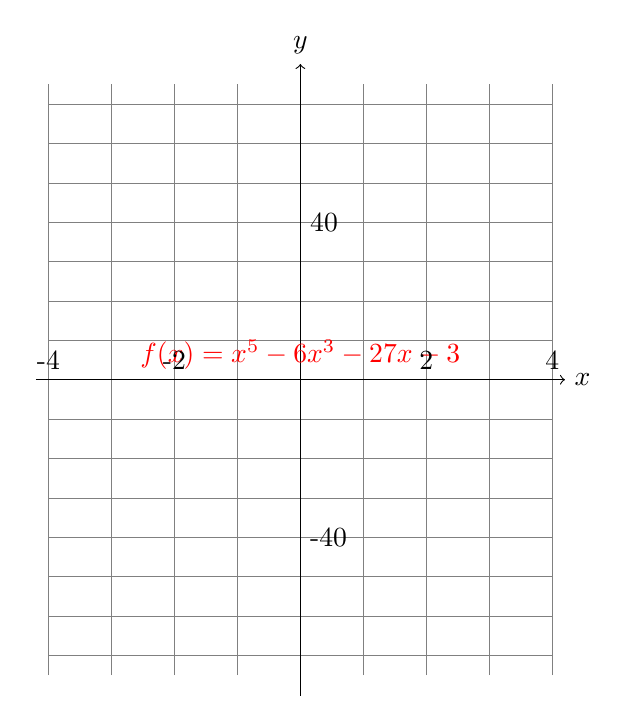
\begin{tikzpicture}[xscale=0.8,yscale=0.05,domain=-3.2:3.2,samples=320]
\draw[very thin,color=gray] (-4,-75) grid [xstep=1,ystep=10] (4,75);

\draw[->] (-4.2,0) -- (4.2,0) node[right] {$x$}; 
\draw[->] (0,-80.2) -- (0,80.2) node[above] {$y$};

\draw[thick,color=red]	plot[smooth,id=quintic]	function{x**5 - 6 *x**3 - 27 *x - 3}	node[above] {$f(x) =x^5 - 6 x^3 - 27 x - 3$};

\node [right] at (0,40)  {40};
\node [right] at (0,-40)  {-40};

\node [above] at (4,0)  {4};
\node [above] at (2,0)  {2};
\node [above] at (-2,0)  {-2};
\node [above] at (-4,0)  {-4};

\end{tikzpicture}


\end{center}
\caption{The graph of $f(x) = x^5 - 6 x^3 - 27 x - 3$}
\label{Galois4}
\end{figure}

 

\begin{example}{galois_x5}
We will show that $f(x) = x^5 - 6 x^3 - 27 x - 3 \in {\mathbb Q}[x]$ is
not solvable. We claim that the Galois group of $f(x)$ over ${\mathbb Q}$
is $S_5$. By Eisenstein's Criterion, $f(x)$ is irreducible and,
therefore, must be separable. The derivative of $f(x)$ is $f'(x) = 5
x^4 - 18 x^2 - 27$; hence, setting $f'(x) = 0$ and solving, we find
that the only real roots of $f'(x)$ are
\[
x = \pm \sqrt{ \frac{6 \sqrt{6} + 9 }{5} }.
\]
Therefore, $f(x)$ can have at most one maximum and one minimum.  It is
easy to show that $f(x)$ changes sign between $-3$ and $-2$, between
$-2$ and $0$, and once again between $0$ and $4$
(Figure~\ref{Galois4}). Therefore, $f(x)$ has exactly three distinct
real roots. The remaining two roots of $f(x)$ must be complex
conjugates. Let $K$ be the splitting field of $f(x)$. Since $f(x)$ has
five distinct roots in $K$ and every automorphism of $K$ fixing ${\mathbb
Q}$ is determined by the way it permutes the roots of $f(x)$, we know
that $G(K/{\mathbb Q})$ is a subgroup of $S_5$. Since $f$ is irreducible,
there is an element in $\sigma \in G(K/{\mathbb Q})$ such that $\sigma(a)
= b$ for two roots $a$ and $b$ of $f(x)$. The automorphism of ${\mathbb
C}$ that takes $a+bi \mapsto a-bi$ leaves the real roots fixed and
interchanges the complex roots; consequently, $G(K/{\mathbb Q} ) \subset
S_5$. By Lemma~\ref{galois:Sn_generating_lemma}, $S_5$ is generated by a transposition and an
element of order 5; therefore, $G(K/{\mathbb Q} )$ must be all of $S_5$. By
Theorem~\ref{normal:An_simple}, $S_5$ is not solvable. Consequently, $f(x)$ cannot be
solved by radicals.  
% Changed $G(K/F )$ to $G(K/{\mathbb Q} )$.  Suggested by Aleks Vlasev. - TWJ 8/10/2011
\end{example}
 
 
 
\subsection*{The Fundamental Theorem of Algebra}
 
 
It seems fitting that the last theorem that we will state and prove
is the Fundamental Theorem of Algebra. This theorem was first proven
by Gauss in his doctoral thesis.  Prior to Gauss's proof, mathematicians 
suspected that there might exist polynomials over the real and complex 
numbers having no solutions. The Fundamental Theorem of Algebra states
that every polynomial over the complex numbers factors into distinct
linear factors. 
 
 
\begin{theorem} \textbf{(Fundamental Theorem of Algebra)}\index{Fundamental
Theorem!of Algebra}
The field of complex numbers is algebraically closed; that is, every
polynomial in ${\mathbb C}[x]$ has a root in ${\mathbb C}$. 
\end{theorem}
 
 
For our proof we shall assume two facts from calculus.  We need the
results that every polynomial of odd degree over ${\mathbb R}$ has a real
root and that every positive real number has a square root.  
 
 
\medskip
 
 
\begin{proof}
Suppose that $E$ is a proper finite field extension of the complex 
numbers. Since any finite extension of a field of characteristic zero
is a simple extension, there exists an $\alpha \in E$ such that $E =
{\mathbb C}( \alpha )$ with $\alpha$ the root of an irreducible
polynomial $f(x)$ in ${\mathbb C}[x]$. The splitting field $L$ of $f(x)$ 
is a finite normal separable extension of ${\mathbb C}$ that contains  $E$.
We must show that it is impossible for $L$ to be a proper extension of
${\mathbb C}$. 
 
 
Suppose that $L$ is a proper extension of ${\mathbb C}$. Since $L$ is the
splitting field of $f(x)(x^2 + 1)$ over ${\mathbb R}$, $L$ is a finite
normal separable extension of ${\mathbb R}$. Let $K$ be the fixed field
of a Sylow 2-subgroup $G$ of $G(L/{\mathbb R})$. Then $L \supset  K
\supset {\mathbb R}$ and $|G( L / K )| =[L:K]$. Since $[L : {\mathbb R}] =
[L:K][K:{\mathbb R}]$, we know that $[K:{\mathbb R}]$ must be odd.
Consequently, $K = {\mathbb R}(\beta)$ with $\beta$ having a minimal
polynomial $f(x)$ of odd degree.  Therefore, $K = {\mathbb R}$. 
 
 
We now know that $G(L/{\mathbb R})$ must be a 2-group. It follows that
$G(L / {\mathbb C})$ is a 2-group.  We have assumed that $L \neq {\mathbb
C}$; therefore, $|G(L / {\mathbb C})| \geq 2$.  By the first Sylow
Theorem and the Fundamental Theorem of Galois Theory, there exists a
subgroup $G$ of $G(L/{\mathbb C})$ of index 2 and a field $E$ fixed
elementwise by $G$. Then $[E:{\mathbb C}] = 2$ and there exists an
element $\gamma \in E$ with minimal polynomial $x^2 + b x + c$ in
${\mathbb C}[x]$.  This polynomial has roots $( - b \pm \sqrt{b^2 - 4
c}\, ) / 2$ that are in ${\mathbb C}$, since $b^2 - 4 c$ is in ${\mathbb
C}$.  This is impossible; hence, $L = {\mathbb C}$.
\end{proof}
 
 
\medskip
 
 
Although our proof was strictly algebraic, we were forced to rely on
results from calculus.  It is necessary to assume the completeness
axiom from analysis to show that every polynomial of odd degree has a
real root and that every positive real number has a square root.  It
seems that there is no possible way to avoid this difficulty and
formulate a purely algebraic argument.  It is somewhat amazing that
there are several elegant proofs of the Fundamental Theorem of Algebra
that use complex analysis.  It is also interesting to note that we can
obtain a proof of such an important theorem from two very different
fields of mathematics. 
 
 
 
\markright{EXERCISES}
\section*{Exercises}
\exrule
 
 
{\small
\begin{enumerate}
 
 
\item
Compute each of the following Galois groups. Which of these field
extensions are normal field extensions? If the extension is not
normal, find a normal extension of ${\mathbb Q}$ in which the extension
field is contained.
\begin{multicols}{2}
\begin{enumerate}

\item 
$G({\mathbb Q}(\sqrt{30}\, ) / {\mathbb Q})$

\item 
$G({\mathbb Q}(\sqrt[4]{5}\, ) / {\mathbb Q})$

\item 
$G( {\mathbb Q}(\sqrt{2}, \sqrt{3}, \sqrt{5}\, )/ {\mathbb Q} )$

\item 
$G({\mathbb Q}(\sqrt{2}, \sqrt[3]{2}, i) / {\mathbb Q})$

\item 
$G({\mathbb Q}(\sqrt{6}, i) / {\mathbb Q})$


\end{enumerate}

\end{multicols}
 

 
 
\item
Determine the separability of each of the following polynomials.
\begin{multicols}{2}
\begin{enumerate}

\item 
$x^3 + 2 x^2 - x - 2$ over ${\mathbb Q}$

\item 
$x^4 + 2 x^2 + 1$ over ${\mathbb Q}$

\item 
$x^4 + x^2 + 1$ over ${\mathbb Z}_3$

\item 
$x^3 +x^2 + 1$ over ${\mathbb Z}_2$

\end{enumerate}
\end{multicols}
 

\item
Give the order and describe a generator of the Galois group of
$\gf(729)$ over~$\gf(9)$.

 
\item
Determine the Galois groups of each of the following polynomials in
${\mathbb Q}[x]$; hence, determine the solvability by radicals of each 
of the polynomials.
\begin{multicols}{2}
\begin{enumerate}

\item 
$x^5 - 12 x^2 + 2$

\item 
$x^5 - 4 x^4 + 2 x + 2$

\item 
$x^3 - 5$

\item 
$x^4 - x^2 - 6$

\item 
$x^5 + 1$

\item 
$(x^2 - 2)(x^2 + 2)$

\item 
$x^8 - 1$

\item 
$x^8 + 1$

\item 
$x^4 - 3 x^2 -10$


\end{enumerate}
\end{multicols}
 
 
 
\item
Find a primitive element in the splitting field of each of the
following polynomials in ${\mathbb Q}[x]$.
\begin{multicols}{2}
\begin{enumerate}

\item 
$x^4 - 1$

\item 
$x^4 - 8 x^2 + 15$

\item 
$x^4 - 2 x^2 - 15$

\item 
$x^3 - 2$

\end{enumerate}
\end{multicols}
  
 
%******************************THEORY*****************
 
 
 
 
\item
Prove that the Galois group of an irreducible quadratic polynomial is
isomorphic to ${\mathbb Z}_2$.
 
 
\item
Prove that the Galois group of an irreducible cubic polynomial is
isomorphic to $S_3$ or ${\mathbb Z}_3$.
 
 
\item
Let $F \subset K \subset E$ be fields. If E is a normal extension of
$F$, show that $E$ must also be a normal extension of $K$.
 
 
\item
Let $G$ be the Galois group of a polynomial of degree $n$.  Prove
that $|G|$ divides~$n!$.
 
 
\item
Let $F \subset E$.  If $f(x)$ is solvable over $F$, show that $f(x)$
is also solvable over $E$.
 
 
\item
Construct a polynomial $f(x)$ in ${\mathbb Q}[x]$ of degree 7 that is not
solvable by \linebreak radicals.
 
 
\item
Let $p$ be prime.  Prove that there exists a polynomial $f(x) \in
{\mathbb Q}[x]$ of degree $p$ with Galois group isomorphic to $S_p$.
Conclude that for each prime $p$ with $p \geq 5$ there exists a
polynomial of degree $p$ that is not solvable by radicals. 
 
 
\item
Let $p$ be a prime and ${\mathbb Z}_p(t)$ be the field of rational
functions over ${\mathbb Z}_p$.  Prove that $f(x) = x^p - t$ is an
irreducible polynomial in ${\mathbb Z}_p(t)[x]$.  Show that $f(x)$ is not
separable. 
 
 
\item
Let $E$ be an extension field of $F$. Suppose that $K$ and $L$ are two 
intermediate fields.  If there exists an element $\sigma \in G(E/F)$
such that $\sigma(K) = L$, then $K$ and $L$ are said to be \boldemph{
conjugate fields}\index{Conjugate fields}\index{Field!conjugate}.
Prove that $K$ and $L$ are conjugate if and only if $G(E/K)$ and
$G(E/L)$ are conjugate subgroups of $G(E/F)$. 
 
 
\item 
Let $\sigma \in \aut( {\mathbb R} )$.  If $a$ is a positive real
number, show that $\sigma( a) > 0$.
 
 
\item 
Let $K$ be the splitting field of $x^3 + x^2 + 1 \in {\mathbb Z}_2[x]$.
Prove or disprove that $K$ is an extension by radicals.
 
\item
Let $F$ be a field such that ${\rm char}\, F \neq 2$. Prove that the
splitting field of $f(x) = a x^2 + b x + c$ is $F( \sqrt{\alpha}\, )$,
where $\alpha = b^2 - 4ac$. 
 
 
\item
Prove or disprove: Two different subgroups of a Galois group will
have different fixed fields.
 
 
 
\item
Let $K$ be the splitting field of a polynomial over $F$. If $E$ is a
field extension of $F$ contained in $K$ and $[E:F] = 2$, then $E$ is
the splitting field of some polynomial in $F[x]$.
 
  
 
\item
We know that the cyclotomic polynomial
\[
\Phi_p(x) = \frac{x^p - 1}{x-1} = x^{p-1} + x^{p-2} + \cdots
+ x + 1
\]
is irreducible over ${\mathbb Q}$ for every prime $p$. Let $\omega$ be a
zero of $\Phi_p(x)$, and consider the field ${\mathbb Q}(\omega)$.
\begin{enumerate}
 
 \item
Show that $\omega, \omega^2, \ldots, \omega^{p-1}$ are distinct zeros of
$\Phi_p(x)$, and conclude that they are all the zeros of $\Phi_p(x)$.
 
 \item
Show that $G( {\mathbb Q}( \omega ) / {\mathbb Q} )$ is abelian of order
$p-1$. 
 
 \item
Show that the fixed field of $G( {\mathbb Q}( \omega ) / {\mathbb Q} )$ is
${\mathbb Q}$. 
 
\end{enumerate}
 
  
\item
Let $F$ be a finite field or a field of characteristic zero.
Let $E$ be a finite normal extension of $F$ with Galois group
$G(E/F)$. Prove that $F \subset K \subset L \subset E$ if and 
only if $\{ id \} \subset G(E/L) \subset G(E/K) \subset G(E/F)$.
 
 
\item
Let $F$ be a field of characteristic zero and let $f(x) \in F[x]$ be
a separable polynomial of degree $n$. If $E$ is the splitting field
of $f(x)$, let $\alpha_1, \ldots, \alpha_n$ be the roots of $f(x)$ in
$E$. Let $\Delta = \prod_{i < j} (\alpha_i - \alpha_j)$.  We
define the \boldemph{discriminant\/}\index{Discriminant!of a separable
polynomial}\label{discriminant} of $f(x)$ to be $\Delta^2$. 
\begin{enumerate}
 
 \item
If $f(x) = x^2 + b x + c$, show that $\Delta^2 = b^2 - 4c$.
 
 \item
If $f(x) = x^3 + p x + q$, show that $\Delta^2 = - 4p^3 - 27q^2$.
 
 \item
Prove that $\Delta^2$ is in $F$.
 
 \item
If $\sigma \in G(E/F)$ is a transposition of two roots of $f(x)$, show
that $\sigma( \Delta )~=~-\Delta$.
 
  \item
If $\sigma \in G(E/F)$ is an even permutation of the roots of $f(x)$, show
that $\sigma( \Delta ) = \Delta$.
 
  \item
Prove that $G(E/F)$ is isomorphic to a subgroup of $A_n$ if and
only if $\Delta \in F$.
 
 \item
Determine the Galois groups of $x^3 + 2 x - 4$ and $x^3 + x -3$.
 
\end{enumerate}

%Exercise corrected and revised.
%TWJ 30/4/2013
 
 
\end{enumerate}
}
 
 
 
 
\subsection*{References and Suggested Readings}
 
{\small
\begin{itemize}
 
\item[\textbf{[1]}] %Reference updated - 21 August 2010 - TWJ
Artin, E. \textit{Theory: Lectures Delivered at the University of Notre Dame (Notre Dame Mathematical Lectures, Number 2)}. 
Dover, Mineola, NY, 1997.
 
\item[\textbf{[2]}]
Edwards, H. M. \textit{Galois Theory}. Springer-Verlag, New
York, 1984.
 
\item[\textbf{[3]}] %Reference updated - 21 August 2010 - TWJ
Fraleigh, J. B. 
\textit{A First Course in Abstract Algebra}. 7th ed.
Pearson, Upper Saddle River, NJ, 2003. 
 
\item[\textbf{[4]}] %Reference updated - 21 August 2010 - TWJ
Gaal, L. \textit{Classical Galois Theory with Examples}. 
American Mathematical Society, Providence, 1979. 
 
\item[\textbf{[5]}]
Garling, D. J. H. \textit{A Course in Galois Theory}.
Cambridge University Press, Cambridge, 1986.
 
 
\item[\textbf{[6]}] %Out of print  - 19 August 2010 - TWJ
Kaplansky, I. \textit{Fields and Rings}. 2nd ed. University of Chicago
Press, Chicago, 1972. 
 
\item[\textbf{[7]}]
Rothman, T. ``The Short Life of \'{E}variste Galois,'' {\it
Scientific American}, April 1982, 136--49.
 
\end{itemize}
}
 
\sagesection
 
